\subsection{Transformers, Indicators, etc.}
\label{subsec:transformers-ind}

Alright, let’s dive into the world of transformers, inductors, and capacitors! These components are the unsung heroes of radio technology, quietly doing their jobs to make sure your circuits work as intended. In this section, we’ll explore resonant circuits, integrated circuits, and the roles of inductors and capacitors. Don’t worry if you’re not an expert—we’ll keep things simple and fun.

\subsubsection*{Resonant Circuits: The Dynamic Duo of Inductors and Capacitors}
A resonant circuit is like a well-choreographed dance between an inductor and a capacitor. When you combine these two components, they create a circuit that can store and release energy at a specific frequency. This is called resonance, and it’s super useful in radio technology for tuning into specific frequencies.

The inductor, with its ability to store energy in a magnetic field, and the capacitor, which stores energy in an electric field, work together to create oscillations. When connected in series or parallel, they form a resonant circuit. The frequency at which this happens is called the resonant frequency, and it’s given by the formula:

\begin{equation}
f = \frac{1}{2\pi\sqrt{LC}}
\label{eq:resonant-frequency}
\end{equation}

Here, \( L \) is the inductance of the inductor, and \( C \) is the capacitance of the capacitor. Pretty neat, right? You can see a diagram of a resonant circuit in Figure~\ref{fig:resonant-circuit}.

\subsubsection*{Integrated Circuits: The Swiss Army Knife of Electronics}
Integrated circuits (ICs) are like the multitaskers of the electronics world. They combine multiple semiconductor devices—like transistors, diodes, and resistors—into a single, compact package. This makes them incredibly versatile and efficient. Whether it’s amplifying a signal, processing data, or controlling a device, ICs are everywhere in modern electronics.

There are different types of ICs, each designed for specific tasks. For example, analog ICs handle continuous signals, while digital ICs work with binary data. You can find a comparison of different IC types in Table~\ref{tab:ics}. And if you’re curious about what an IC looks like on the inside, check out Figure~\ref{fig:ic}.

\subsubsection*{Inductors and Capacitors: The Yin and Yang of Circuits}
Inductors and capacitors are like the yin and yang of electronic components. Inductors resist changes in current, while capacitors resist changes in voltage. Together, they form the backbone of many circuits, including the resonant circuits we just talked about.

An inductor’s primary job is to store energy in a magnetic field when current flows through it. This stored energy can then be released back into the circuit, which is why inductors are often used to smooth out current fluctuations. Capacitors, on the other hand, store energy in an electric field and are great for filtering out noise or stabilizing voltage.

\subsubsection*{Questions}
\begin{tcolorbox}[colback=gray!10!white,colframe=black!75!black,title={T6D08}]
Which of the following is combined with an inductor to make a resonant circuit?
\begin{enumerate}[label=\Alph*),noitemsep]
    \item Resistor
    \item Zener diode
    \item Potentiometer
    \item \textbf{Capacitor}
\end{enumerate}
\end{tcolorbox}
A resonant circuit is made by combining an inductor and a capacitor. The inductor stores energy in a magnetic field, while the capacitor stores energy in an electric field. Together, they create oscillations at a specific frequency, known as the resonant frequency. The other options—resistor, Zener diode, and potentiometer—don’t play a role in creating resonance.

\begin{tcolorbox}[colback=gray!10!white,colframe=black!75!black,title={T6D09}]
What is the name of a device that combines several semiconductors and other components into one package?
\begin{enumerate}[label=\Alph*),noitemsep]
    \item Transducer
    \item Multi-pole relay
    \item \textbf{Integrated circuit}
    \item Transformer
\end{enumerate}
\end{tcolorbox}
An integrated circuit (IC) is a device that combines multiple semiconductor components, like transistors and diodes, into a single package. This makes ICs incredibly versatile and efficient for a wide range of applications. The other options—transducer, multi-pole relay, and transformer—don’t fit this description.

\begin{tcolorbox}[
    colback=gray!10!white,
    colframe=black!75!black,
    title={T6D10},
    sidebyside,
    sidebyside align=top,
    lefthand width=0.45\textwidth
]
What is the function of component 2 in figure T-1?
\begin{enumerate}[label=\Alph*),noitemsep]
    \item Give off light when current flows through it
    \item Supply electrical energy
    \item \textbf{Control the flow of current}
    \item Convert electrical energy into radio waves
\end{enumerate}
\tcblower
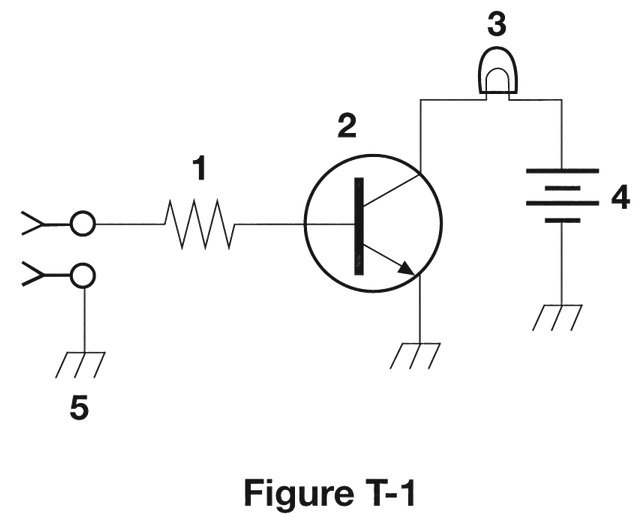
\includegraphics[width=0.7\textwidth]{tech/images/t1.png}
\end{tcolorbox}
Component 2 in Figure T-1 is an inductor, which is used to control the flow of current in a circuit. Inductors store energy in a magnetic field and resist changes in current, making them ideal for smoothing out current fluctuations. The other options don’t describe the function of an inductor.

\begin{tcolorbox}[colback=gray!10!white,colframe=black!75!black,title={T6D11}]
Which of the following is a resonant or tuned circuit?
\begin{enumerate}[label=\Alph*),noitemsep]
    \item \textbf{An inductor and a capacitor in series or parallel}
    \item A linear voltage regulator
    \item A resistor circuit used for reducing standing wave ratio
    \item A circuit designed to provide high-fidelity audio
\end{enumerate}
\end{tcolorbox}
A resonant or tuned circuit is made by combining an inductor and a capacitor in series or parallel. This combination allows the circuit to oscillate at a specific frequency, which is useful for tuning into radio frequencies. The other options—linear voltage regulator, resistor circuit, and high-fidelity audio circuit—don’t create resonance.

\subsubsection*{Figures and Tables}
% Figure: Resonant circuit with inductor and capacitor
\begin{figure}[h!]
    \centering
    %\includegraphics[width=0.6\textwidth]{resonant-circuit.svg} % Placeholder for the image
    \caption{Resonant circuit with inductor and capacitor.}
    \label{fig:resonant-circuit}
    % Image prompt: Diagram of a resonant circuit with an inductor and capacitor.
\end{figure}

% Figure: Integrated circuit schematic
\begin{figure}[h!]
    \centering
    %\includegraphics[width=0.6\textwidth]{ic.svg} % Placeholder for the image
    \caption{Integrated circuit schematic.}
    \label{fig:ic}
    % Image prompt: Schematic of an integrated circuit.
\end{figure}

% Table: Comparison of integrated circuit types
\begin{table}[h!]
    \centering
    \begin{tabular}{|l|l|}
        \hline
        \textbf{Type} & \textbf{Description} \\
        \hline
        Analog IC & Handles continuous signals \\
        Digital IC & Works with binary data \\
        Mixed-Signal IC & Combines analog and digital functions \\
        \hline
    \end{tabular}
    \caption{Comparison of integrated circuit types.}
    \label{tab:ics}
    % Table prompt: Table comparing different types of integrated circuits.
\end{table}
